\chapter{Implementation and Performance Analysis}

\section{Analysis of Naive Template Matching}
In this section, we'll analyze the implementation and the performance of the \textit{Naive Template Matching} algorithm. First of all, let's consider the serial implementation case. 

\subsection{Bitmap Images}
For this project, we've used the \textit{bitmap} image library by \textit{Arash Partow} which is accessible \href{https://github.com/ArashPartow/bitmap}{here}.

\subsection{Serial Implementation of NTM}
The serial implementation of this algorithm consists of 2 main loops to iterate over image pixels. There is also a need for each pixel we are iterating through, to calculate the \textit{Sum of Absolute Deviations} which is the similarity measure between the main image pixels and the template image. Please refer to the \textit{Naive Template Matching} algorithm to see the code. Since the task is mainly focused on counting the number of occurance inside the main images, we can obtain this by finding the minimum value of \textit{SAD} while iterating through the main image pixels and counting the number of occurrences of the found minimum inside the main image matrix.

\subsection{Timing the Serial NTM}
We can obtain the elapsed time for the serial iteration using the \textit{chrono} library. The code for this section is provided here. Please refer to the serial implementation code for the details. 

\subsection{CUDA Implementation of NTM}
In this section we'll walk through the kernel codes provided in the \textit{kernel.cu}.
\subsubsection{Compute Sad Array Kernel}
The image data is being stored in an 1-D array. Thus, the best choice for CUDA kernel launch parameters would be to set grid dimensions as $(image\_width/block\_size\_x, image\_height/block\_size\_y, 1)$. The main purpose of this choice is not the way we have stored the data, it actually depends on the input data. Since we are dealing with images it is more suitable to have 2-D blocks of threads. Further explanations focus on the kernel implementation. Initially, each thread finds its own global 2-D identification as rows and columns. Then, each thread virtually sees a kernel (template) around it self. This is the core of the parallelization section. All threads can see all of the iterations in one place. We then compute the SAD of each pixel and load it inside an SAD array. The next section describes the reason to do so.

\subsubsection{Find Minimum in Array Kernel}
We can obtain the best possible match by finding the minimum SAD in SAD array. We'll do so using shared memory to speed up the process. Each thread helps loading the data inside a block into the shared memory of that block. We then use \textit{fminf} to find the minimum inside each block. Since we are using the shared memory, we need to do a \textit{reduction} to find the minimum across different blocks. We can obtain this reduction task defining a \textit{mutex} to control the global memory write by first thread of each block.

\subsubsection{Find Number of Occurrences}
Since the main task is to find the number of occurrences of template image in main image, we should count the number of occurrences of minimum SAD in the SAD array. To speed up the process we've used shared memory again. The intuition of using shared memory is exactly the same as the previous section.

\subsection{Launch Parameters on Test Cases}
The test has been done on three different sizes of images. One of the medium sized images is a \textit{bitmap} image with dimensionality of $1112 * 1500$. The template image is a $116*116$ image in this case. Considering a block size of 1024 on a \textit{Nvidia 850m GTX} (compute capability of 5), the launch parameters are provided below:
\begin{figure}[!h]\centering
	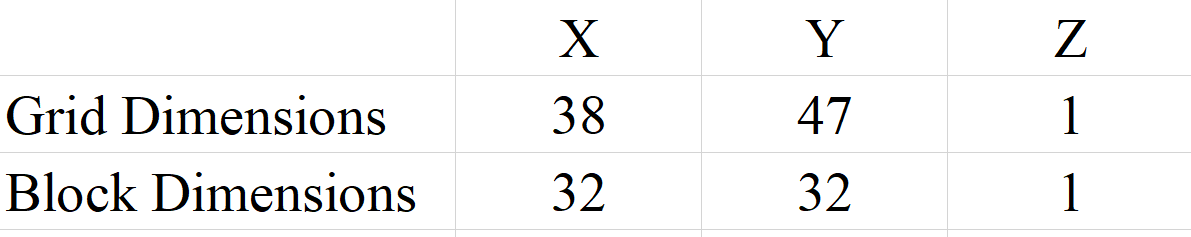
\includegraphics[width=0.6\textwidth]{grid_block.PNG}
	\label{pl1}
\end{figure}

\subsection{Occupancy Analysis}
Before getting into the details, it is important to mention that maximum number of active warps in theory is 64. \textit{Nsight} profiler provides great details on the number of active warps per SM. In this case, there are 63.83 active warps on the first kernel (Compute Sad Array Kernel). The occupancy can obtained by dividing the number of active warps to the number of maximum warps available:
\begin{equation}
	 occupancy = \frac{63.83}{64} = 99.74 \%
\end{equation}
\begin{figure}[!h]\centering
	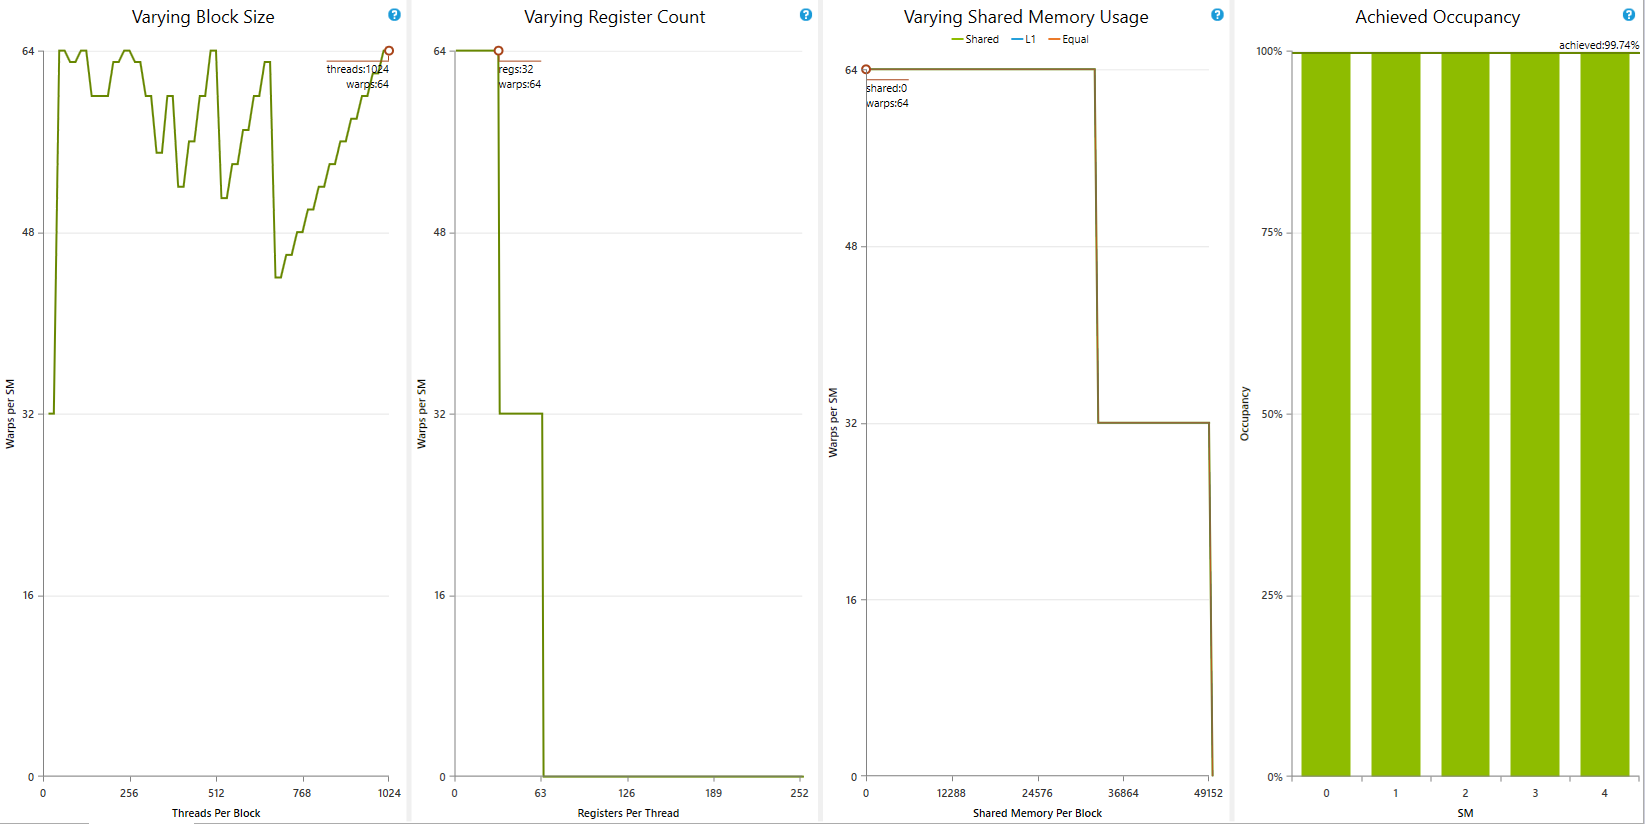
\includegraphics[width=0.99\textwidth]{occupancy_analysis.PNG}
	\caption{Illustration of varying the size of blocks, registers and shared memory on the achieved occupancy.}
	\label{pl1}
\end{figure}

According to figure 3.1, varying the number of threads per block might yield the same result in other scenarios. The circled point shows the current number of threads per block and the current upper limit of active warps. Note that the number of active warps is not the number of warps per block (that is threads per block divided by warp size, rounded up). If the chart's line goes higher than the circle, changing the block size could increase occupancy without changing the other factors.  Also, increasing the number of variables (registers per block) will drastically decrease the occupancy of the first kernel.

\subsection{SM Activity Analysis}
\begin{figure}[!h]\centering
	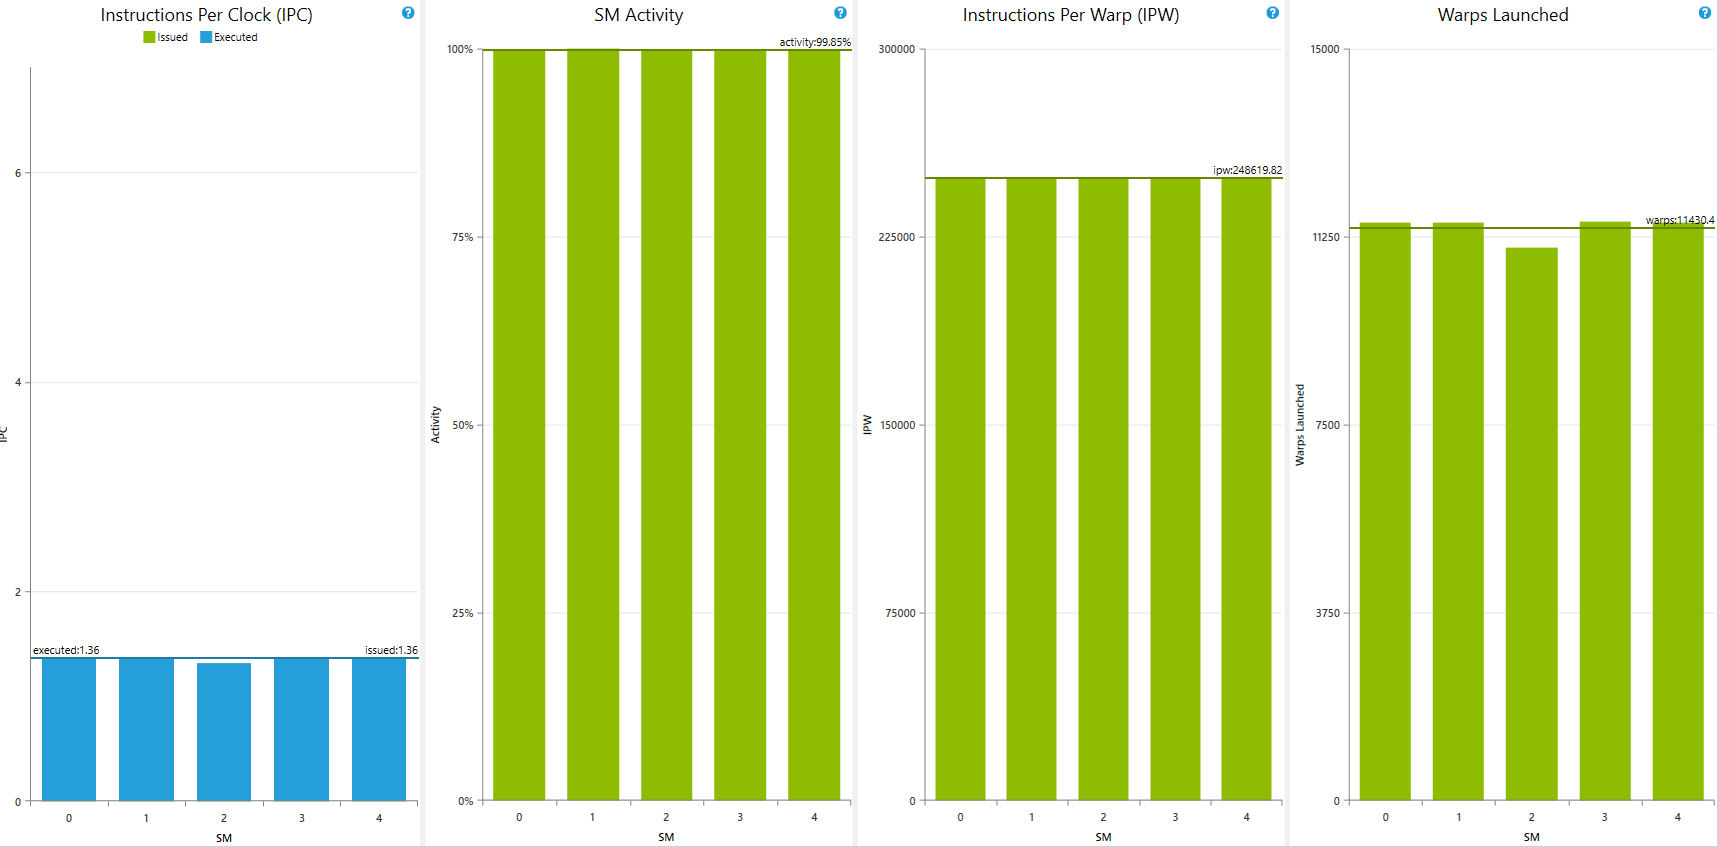
\includegraphics[width=0.99\textwidth]{sm_activity.PNG}
	\caption{Issue efficiency and SM activity charts for the first (bottleneck) kernel.}
	\label{pl1}
\end{figure}
The IPC chart demonstrates the achieved instructions throughputs per SM for both, issued instructions and executed instructions. The theoretical maximum peak IPC is a device limit and defined by the compute capabilities of the target device.

\subsubsection{Issued IPC}
The average number of issued instructions per cycle accounting for every iteration of instruction replays. Optimal if as close as possible to the Executed IPC. As described in the background section of this document, some assembly instructions require to be multi-issued. Hence, the instruction mix affects the definition of the optimal target for this metric. In this case, the issued IPC throughput is minimum since there weren't any multi issue instructions in the first kernel.

\subsubsection{Executed IPC}
The average number of executed instructions per cycle. Each warp scheduler of a multiprocessor can execute instructions independently, a target goal of executing one instruction per cycle means executing on average with an IPC equal to the number of warp schedulers per SM. The maximum achievable target IPC for a kernel is dependent on the mixture of instructions executed. 

\subsubsection{SM Activity Chart}
The second chart provides information on the activity of each SM during the kernel launch. A multiprocessor is considered to be active if at least one warp is currently assigned for execution. An SM can be inactive - even though the kernel grid is not yet completed - due to high workload imbalances. Such uneven balancing between the SMs can be caused by a few factors: Different execution times for the kernel blocks, variations between the number of scheduled blocks per SM, or a combination of the two. In this case, non of the above has occurred and the activity result is almost 100\%.

\subsubsection{IPW Chart}
One of the most common patterns for varying IPWs is conditionally executed code blocks. IPW can be useful while having variations in SM activity chart which in this case, non of these have occurred.

\subsection{Speedup Analysis}
In this section, we'll analyze the possible theoretical speedup. For this purpose, we'll calculate the serial computation time for the \textit{collection} and \textit{collection\_coin} images as described above. This table describes the average speedup of parallel naive template matching algorithm compared to serial implementation. As can be seen in the figure 3.3, the speedup obtained on GPU is dedicated to many different parameters. In order to calculate the theoretical speedup a direct use of \textit{Amdahl's law} doesn't fit in this problem. One might say that the number of cores in this case is \textit{N} (Same as the number of threads), but GPU does not have as many physical cores as the number of threads that can be launched. Additionally, significant portion of kernel time is begin spent just waiting for the data to be \textit{read/written} from/to global memory. Also, the frequency and operational power of CPU cores is higher than GPU cores. In this section, we'll use a modified version of the Amdahl's law \cite{amdahl}:
\begin{equation}
	S = \frac{1}{(1 - p) + (k * p / N)} \ \ \ \ \  \ k = freq(CPU) / freq(GPU)
\end{equation}
The core frequency of my Intel 4710HQ processor is 3490 MHz. The core frequency of each GPU core is 902 MHz. These information are extracted using beloved \textit{CPU-Z} and \textit{GPU-Z} programs. Replacing these information into 3.2 yields
\begin{equation}
	S = \frac{1}{(1 - p) + 3.86 * p / N}
\end{equation}
since the size of input is constant in this law, we'll assume that 3.3 is correct for the third experiment. Let's suppose that $\frac{1}{4}$ of the main program is parallelized, thus $p = \frac{1}{4}$ and the number of threads to run is 1828864 (1786 blocks of 1024). Theoretical speedup will be
\begin{equation}
	S = \frac{1}{(\frac{3}{4}) + 3.86 * \frac{\frac{1}{4}}{1828864}} = 1.33
\end{equation}
\begin{figure}[!h]\centering
	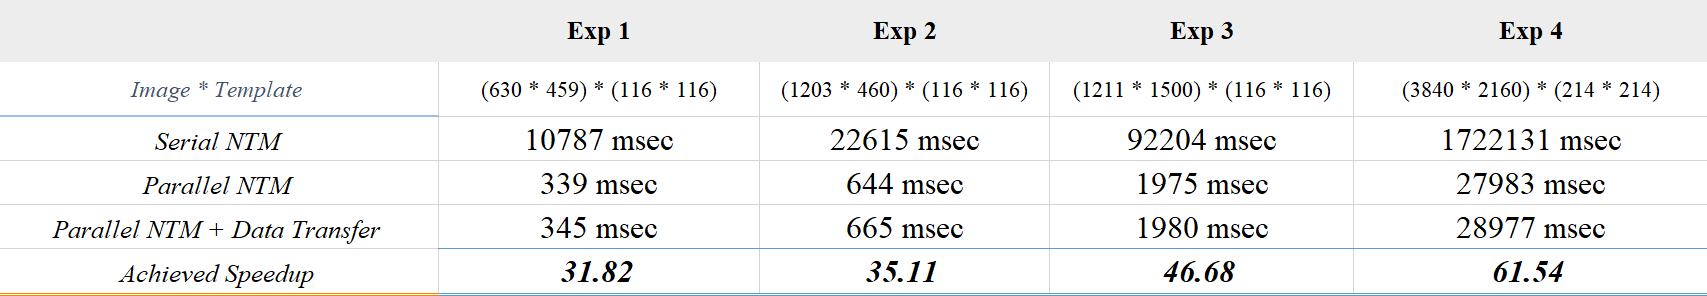
\includegraphics[width=0.99\textwidth]{speedup.PNG}
	\caption{Computation and data transfer time for naive serial and parallel implementation.}
	\label{pl1}
\end{figure}

\subsection{Performance Analysis}
In this section, we'll analyze the performance of the \textit{Compute Sad Array Kernel}. Firstly, lets find the arithmetic intensity of this kernel. Arithmetic intensity $I$, also called \textit{operational intensity}, is the ratio of \textit{arithmetic operations} or \textit{work} ($W$), to the \textit{memory traffic} ($Q$) \cite{roofline}:
\begin{equation}
	I = \frac{W}{Q}
\end{equation}
and denotes the number of operations per byte of memory traffic. When the work is represented as \textit{FLOPS}, the arithmetic intensity will be \textit{FLOPS/Byte}. According to the \textit{Naive Roofline Model}, the \textit{attainable performance} is bound either by the \textit{peak performance} or \textit{memory bandwidth * arithmetic intensity}. In this case, the operational intensity can be obtained by following the memory access patterns and the work being done in the main kernel:
\begin{figure}[!h]\centering
	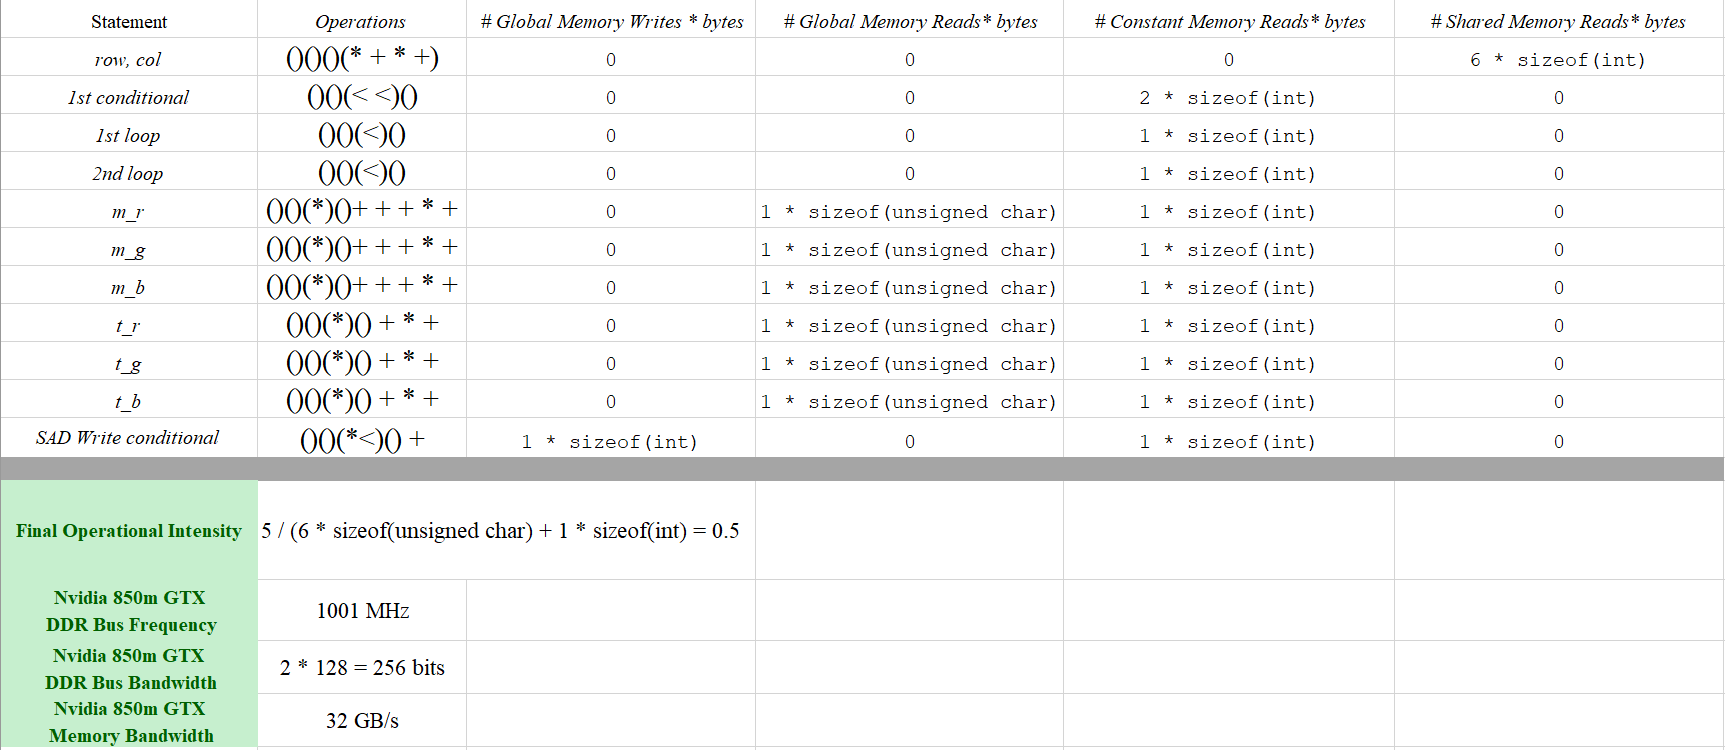
\includegraphics[width=1\textwidth]{intensity.PNG}
	\caption{Calculation of first kernel operational intensity and GPU memory bandwidth.}
	\label{pl1}
\end{figure}
It is given that the \textit{single precision} processing power of a \textit{Nvidia 850m GTX} is 1155 GFLOPS \cite{techpower}. Given these results, the kernel is actually memory bound since $0.5 < 1155 / 32 = 36$. The kernel arithmetic intensity should be at least 36 to be considered a compute bound kernel.

\section{Implementation of FFT Based Template Matching}
In this section, we delve into the details of \textit{FFT} based template matching using \textit{cufft} library from \textit{Nvidia}. Note that this implementation is still in progress and there are multiple serial loops conducted in preprocessing step which slows down the process compared to the \textit{naive template matching} procedure.
As mentioned before, the overall procedure is to convert the spatial domain of input images to the frequency domain. In the frequency domain, we can apply a correlation based operation. This operation yields a signal of the same size as main image size. We then apply an inverse Fourier transform to turn the results back to the spatial domain. We then find the maximum of that signal and the number of occurrences of that maximum value in that signal. The procedure is well defined below\cite{gonzalez}:
\begin{equation}
	c = real(IFFT_{2D} (FFT_{2D}(main\_image) .* FFT_{2D}(template\_image)))
\end{equation}	
according to 3.6, $c$ contains a list of values which we are desired to find the maximum of it (for maximum similarity). To obtain this in CUDA, we've used multiple functions which are described further. Note that \textit{*} symbol shows the complex conjugate of the second signal.

\subsection{Real to Complex Conversion}
For this part, we have not focused on the performance. We use simple \textit{for} loops to convert the image data matrix to the proper format of \textit{cufft} library which is called \textit{cufftComplex}. \textit{cufftComplex} is a simple typedef of \textit{float} type in C.

\subsection{Padding Data}
Before performing a \textit{2-D Forward Fourier Transform} we are urged to perform a data padding on template signal to make it the same size as the main signal. Figure 2.1 illustrates this phenomenon pretty well. The duty of data padding is simple. Allocate new memory with a new size. Copy signals into their corresponding location in new allocated memory and set other places to 0.

\subsection{2-D FFT Planning}
\textit{cufft} library uses the concept of \textit{plan} to provide the baseline setup for the main APIs provided in the library. A plan can initiate a 1-D, 2-D or 3-D data processing API from \textit{cufft} library. In this implementation, we need a setup for a 2 dimensional Fourier transform, thus we use \textit{cufftPlan2d} to prepare the library for the main transformations.

\subsection{Forward FFT Launch}
In order to launch a forward \textit{complex to complex} Fourier transform using \textit{cufft}, we'll use \textit{cufftExecC2C}. The constant \textit{CUFFT\_FORWARD} shows the direction of the Fourier transform which is \textit{Forward} in this case.

\subsection{Complex Conjugate Kernel}
This kernel implements the conjugation procedure. The implementation is pretty straightforward. Each thread multiples the corresponding signal point's complex part to -1 and loads it back to the input signal.

\subsection{Complex Point-wise Kernel}
This kernel provides a point to point multiplication manner for each of the points in main and template input signals. It uses another kernel called \textit{ComplexMul} to perform a \textit{complex multiplication}. It then scales the result using \textit{ComplexScale}. Scaling or normalization is mainly done by dividing the signal values to the size of the signal.

\subsection{Inverse FFT Launch}
Finally, we'll perform an inverse Fourier transform on the result of the \textit{Complex Point-wise Kernel}. The resulting signal is in the spatial domain.

\subsection{Get Maximum and Number of Occurrences}
To find the number of occurrences, we \textit{serially} iterate over the resulting signal of the previous section. Note that these steps are not \textit{100\%} efficient and are still in improvement.